\documentclass{rvcepaper}
\newcommand{\orrow}{\multicolumn{6}{|c|}{\bfseries OR}\\ \hline}
\newcommand{\instrA}[1]{\begin{seeinstr}\item Answer all questions from Part A. Part A questions should be answered in first three pages of the answer book only.\item Answer FIVE full questions from Part B. In Part B question number 2 is compulsory. Answer any one full question from 3 and 4, 5 and 6, 7 and 8, 9 and 10.#1\end{seeinstr}}
\newcommand{\lgrid}{%
\par\vspace{4pt}\centerline{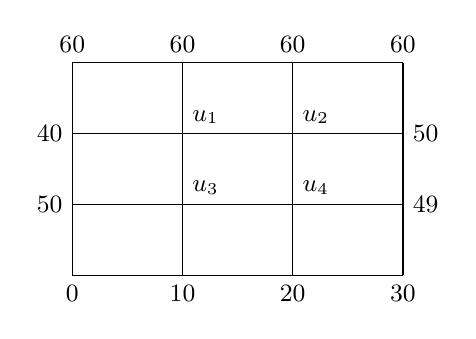
\begin{tikzpicture}[x=1.4cm,y=0.9cm]
 \foreach \i in {0,1,2,3}{\draw (\i,0)--(\i,3); \draw (0,\i)--(3,\i);}
 \foreach \x in {0,1,2,3}{\node[above] at (\x,3) {\small 60};}
 \node[left] at (0,2) {\small 40}; \node[left] at (0,1) {\small 50}; \node[right] at (3,2) {\small 50}; \node[right] at (3,1) {\small 49};
 \node[below] at (0,0) {\small 0}; \node[below] at (1,0) {\small 10}; \node[below] at (2,0) {\small 20}; \node[below] at (3,0) {\small 30};
 \node at (1,2) [above right] {\small $u_1$}; \node at (2,2) [above right] {\small $u_2$}; \node at (1,1) [above right] {\small $u_3$}; \node at (2,1) [above right] {\small $u_4$};
\end{tikzpicture}}\par\centerline{\small Fig 9a}\par\vspace{2pt}}
\begin{document}

%%%%%%%%%%%%%%%%%%%%%%%%%%%%%%%%%%%%%%%% MATHEMATICS
% ---------------- MA231TB, April 2024
\begin{seepaper}
\paperinfo{code={MA231TB},examline={III Semester B.E. Examinations April -- 2024 \\ Common to AS, BT, CH, IEM, ME},dept={Department of Mathematics},title={STATISTICS, LAPLACE TRANSFORM AND NUMERICAL METHODS},time={03 Hours},maxmarks={100}}
\seehead
\instrA{\item Use of scientific calculator and hand book for mathematics is permitted.}
\seepartA
\begin{seeA}
\qaq{1}{1.1}{If the first four moments of a distribution about the value 25 of the variables are $-3, 11, -29$ and 71, then the second moment about the mean is \blank[1.5cm].}{02}{1}{2}
\qa{1.2}{The equations of regression lines are y = 0.5x + 1 and x = 0.4y + 3. The correlation coefficient is \blank[1.5cm].}{02}{2}{2}
\qa{1.3}{The real part of the complex function $f(z) = \log_e z$ in cartesian co-ordinate system is \blank[1.5cm].}{02}{1}{1}
\qa{1.4}{Taylor's series expansion of $\cos z$ about the point $z = \pi/4$ is \blank[1.5cm].}{02}{2}{1}
\qa{1.5}{The Laplace transform of the signal $f(t) = t + \cos 2t$ is \blank[1.5cm].}{02}{1}{1}
\qa{1.6}{Region of convergence of $\mathcal{L}[a^t]$ to hold good is \blank[1.5cm].}{02}{1}{1}
\qa{1.7}{$\mathcal{L}^{-1}\left[\dfrac{1}{4s-1}\right]$ = \blank[1.5cm].}{02}{1}{2}
\qa{1.8}{If $F(s) = \dfrac{1}{s^2+4s+4}$, then the inverse Laplace transform of $F(s)$ = \blank[1.5cm].}{02}{2}{1}
\qa{1.9}{The equation $u_{xx} + u_{yy} - 4u_x - 6u_y = 3$ is classified as \blank[1.5cm].}{02}{1}{1}
\qa{1.10}{For the one dimensional wave equation $u_{xx} = u_{tt}$ with the boundary conditions $u(0,t) = 0$, $u(1,t) = 0$, $u_t(x,0) = 0$ and $u(x,0) = x - x^2$, the value of $u(0.25, 0.25)$ by taking h = 0.25 and k = 0.25 is \blank[1.5cm].}{02}{2}{2}
\end{seeA}
\seepart{PART-B}
\begin{seeB}
\qb{2}{a}{From the following frequency distribution, compute first three moments about the mean.
\qtabc{|c|*{6}{c|}}{\hline x & 1 & 2 & 3 & 4 & 5 & 6\\\hline y & 1 & 6 & 13 & 25 & 30 & 22\\\hline}}{05}{2}{3}
 & b & A simply supported beam carries a concentrated load P at its mid-point. Corresponding to various values of P, the maximum deflection Y is measured and is given in the following table.
\qtabc{|c|*{6}{c|}}{\hline P & 100 & 120 & 140 & 160 & 180 & 200\\\hline Y & 0.45 & 0.55 & 0.60 & 0.70 & 0.80 & 0.85\\\hline}
Fit a law of the form Y = a + bP and hence estimate Y when P is 150. & 06 & 3 & 2\\ \hline
 & c & Calculate the rank correlation coefficient from the following data:
\qtabc{|c|*{8}{c|}}{\hline x & 81 & 78 & 73 & 73 & 69 & 68 & 62 & 58\\\hline y & 10 & 12 & 18 & 18 & 18 & 22 & 20 & 24\\\hline} & 05 & 3 & 3\\ \hline
\qb{3}{a}{Determine the analytic function whose real part is $u = e^x(x\cos y - y\sin y)$ by Milne-Thomson method. Also find its harmonic conjugate v.}{08}{2}{2}
 & b & Obtain the Laurent's series expansion for $f(z) = \dfrac{1}{(z+1)(z+3)}$ in the region (i) $1 < |z| < 3$ (ii) $|z| > 3$ (iii) $|z| < 1$. & 08 & 2 & 2\\ \hline
\orrow
\qb{4}{a}{Find the analytic function $f(z) = u + iv$ where $u - v = 2xy + x^2 - y^2 + x - y$.}{08}{2}{2}
 & b & Evaluate the integral $\displaystyle\int_C \dfrac{e^{2z}}{(z+1)(z-2)^2}\,dz$ where C is the circle $|z| = 3$ using Cauchy's residue theorem. & 08 & 2 & 2\\ \hline
\qb{5}{a}{A periodic function f(t) of period 2a, a $>$ 0 is defined by $f(t) = K$ for $0 \le t \le a$ and $-K$ for $a < t \le 2a$. Show that $\mathcal{L}\{f(t)\} = \dfrac{K}{s}\tanh\left(\dfrac{as}{2}\right)$.}{08}{2}{2}
 & b & Obtain the Laplace transform of $\dfrac{e^{-t} - e^{7t}}{t} + \left(2\sqrt{t} - \dfrac{3}{\sqrt{t}}\right)^3$. & 08 & 3 & 3\\ \hline
\orrow
\qb{6}{a}{Express the following in terms of unit step function and hence find the Laplace transform of $f(t) = \begin{cases}3t^2, & 0 < t < 3\\ 5t, & t > 3\end{cases}$}{08}{2}{2}
 & b & Find $\mathcal{L}\left\{e^{-t}\left(\int_0^t t\sin 4t\,dt\right) + \cos 2t\sin 5t\right\}$. & 08 & 3 & 3\\ \hline
\qb{7}{a}{The signal in frequency domain is given by $\dfrac{s}{(s-3)(s^2+4)}$. Determine the transformation in time domain.}{08}{2}{3}
 & b & Employing convolution theorem, find inverse Laplace transform of $\dfrac{1}{(s^2+a^2)^2}$. & 08 & 3 & 4\\ \hline
\orrow
\qb{8}{a}{Evaluate $\mathcal{L}^{-1}\left[\dfrac{s+1}{s^2-s+1}\right]$.}{08}{2}{3}
 & b & Solve the differential equation using Laplace transform $\dfrac{d^2y}{dt^2} - 3\dfrac{dy}{dt} + 2y = 12e^{-t}$ when $y(0) = 2$ and $y'(0) = 6$. & 08 & 3 & 4\\ \hline
\qb{9}{a}{Determine the value of $u(x,y)$ satisfying the Laplace equation $\dfrac{\partial^2u}{\partial x^2} + \dfrac{\partial^2u}{\partial y^2} = 0$ at the pivotal points of a square region with boundary values as shown in Fig 9a. Carry out 3 iterations.
\lgrid}{08}{2}{4}
 & b & Employ Bendre-Schmidt method with h = 1 to find the values of $u(x,t)$ up to t = 1 for the equation $2\dfrac{\partial^2u}{\partial x^2} = \dfrac{\partial u}{\partial t}$, $0 < x < 4$, $t > 0$ under the conditions $u(x,0) = x(4-x)$, $0 < x < 4$; $u(0,t) = u(4,t) = 0$, $t \ge 0$. & 08 & 3 & 3\\ \hline
\orrow
\qb{10}{a}{The temperature distribution $u(x,t)$ is modeled as the one-dimensional heat equation $\dfrac{\partial u}{\partial t} = \dfrac{4}{5}\dfrac{\partial^2u}{\partial x^2}$, $0 < x < 100$, $t > 0$ subject to the boundary conditions $u(0,t) = 0 = u(100,t)$, $t \ge 0$ and the initial condition $u(x,0) = x$ for $0 \le x \le 50$ and $100 - x$ for $50 \le x \le 100$. Determine the temperature distribution $u(x,t)$ by taking h = 20 and k = 10 using Schmidt relation for 5 levels.}{08}{2}{3}
 & b & Solve $\dfrac{\partial^2u}{\partial t^2} = 16\dfrac{\partial^2u}{\partial x^2}$ taking h = 1 in five steps given that $u(x,0) = x^2(5-x)$, $u_t(x,0) = 0$, $u(0,t) = u(5,t) = 0$. & 08 & 3 & 4\\ \hline
\end{seeB}
\end{seepaper}

% ---------------- MA231TB, Model Question Paper (2022 scheme)
\begin{seepaper}
\paperinfo{code={MA231TB},examline={III Semester B.E. April -- 2024 Examinations \\ Common to AS, BT, CH, IEM, ME \\ MODEL QUESTION PAPER (2022 SCHEME)},dept={Department of Mathematics},title={STATISTICS, LAPLACE TRANSFORMS AND NUMERICAL METHODS},time={03 Hours},maxmarks={100}}
\seehead
\instrA{}
\seepartA
\begin{seeA}
\qaq{1}{1.1}{A frequency distribution curve is said to be `platykurtic' if \blank[2cm].}{01}{--}{--}
\qa{1.2}{If two variables x and y are perfectly correlated then, coefficient of correlation `r' is \blank[1.8cm].}{01}{--}{--}
\qa{1.3}{If the equations of regression lines of two variables x and y are x $-$ y = 0, 4x $-$ y = 3 then the means of x and y are \blank[1.2cm] and \blank[1.2cm].}{02}{--}{--}
\qa{1.5}{The real and imaginary parts of the function $f(z) = z + e^z$ is \blank[1.2cm] and \blank[1.2cm].}{02}{--}{--}
\qa{1.6}{The residue of $f(z) = \dfrac{1}{(z+2)(z+3)}$ at the pole z = 3 is \blank[1.8cm].}{02}{--}{--}
\qa{1.7}{Compute: $\mathcal{L}[e^{3t}\cosh(2t)]$ is \blank[1.8cm].}{02}{--}{--}
\qa{1.8}{The Laplace transform of the signal $f(t) = t\,\delta(t-3)$ is \blank[1.8cm].}{02}{--}{--}
\qa{1.9}{Evaluate: $\mathcal{L}^{-1}\left[\dfrac{3}{s^2-4}\right]$.}{02}{--}{--}
\qa{1.10}{If $F(s) = \dfrac{1}{s^2+2s+7}$, then $\mathcal{L}^{-1}[F(s)]$ = \blank[1.8cm].}{02}{--}{--}
\qa{1.11}{The forward difference approximation for $u_t$ and central difference approximation $u_x$ are \blank[1.5cm] and \blank[1.5cm].}{02}{--}{--}
\qa{1.12}{The 1D wave equation $c^2u_{xx} - u_{tt} = 0$ is classified as \blank[1.8cm].}{02}{--}{--}
\end{seeA}
\seepart{PART-B}
\begin{seeB}
\qb{2}{a}{Compute the first four moments about the mean of the frequency distribution given below:
\qtabc{|l|*{5}{c|}}{\hline x & 0 & 1 & 2 & 3 & 4\\\hline f & 1 & 8 & 28 & 56 & 70\\\hline}}{10}{--}{--}
 & b & The following table gives ranking of 10 students according to their achievements in both the laboratory and lecture portions of an engineering course. Find the coefficient of rank correlation.
\qtabc{|l|*{10}{c|}}{\hline Lab (x) & 8 & 3 & 9 & 2 & 7 & 10 & 4 & 6 & 1 & 5\\\hline Lecture (y) & 9 & 5 & 10 & 1 & 8 & 7 & 3 & 4 & 2 & 6\\\hline} & 6 & -- & --\\ \hline
\qb{3}{a}{Show that the function $f(z) = z^2$ is analytic and hence obtain its derivative.}{8}{--}{--}
 & b & Expand the function $f(z) = \dfrac{z}{(z+1)(z+3)}$ as power series in the region $1 < |z| < 3$. & 8 & -- & --\\ \hline
\orrow
\qb{4}{a}{Construct an analytic function $f(z) = u + iv$, if the real part of the function is $u = x^2 + x - y^2$.}{8}{--}{--}
 & b & Evaluate $\displaystyle\int_C \dfrac{3z-4}{z(z-1)(z-2)}\,dz$ by using the residue theorem if C: $|z|$ = 3/2. & 8 & -- & --\\ \hline
\qb{5}{a}{For the periodic function $f(t) = \begin{cases}1, & 0 < t < \frac{a}{2}\\ -1, & \frac{a}{2} < t < a\end{cases}$, where $f(t+a) = f(t)$, find $\mathcal{L}[f(t)]$. Sketch the graph of the function.}{8}{--}{--}
 & b & Find (i) $\mathcal{L}[te^{-3t} + \sin(t)\sin(3t)]$ (ii) $\mathcal{L}\left[\dfrac{\sin(2t)}{t}\right]$. & 8 & -- & --\\ \hline
\orrow
\qb{6}{a}{Evaluate: $\mathcal{L}\left[\left(2\sqrt{t} - \dfrac{1}{3\sqrt{t}}\right)^3 + t\cos(2t)\right]$.}{8}{--}{--}
 & b & Express the function in terms of unit step function and hence, obtain the Laplace transform of $f(t) = \begin{cases}\cos(t), & 0 < t < \pi\\ 1, & \pi < t \le 2\pi\\ \sin(t), & t \ge 2\pi\end{cases}$ & 8 & -- & --\\ \hline
\qb{7}{a}{Find the inverse Laplace transform of the following: (i) $\dfrac{3s+2}{2s^2-4s+3}$ (ii) $\dfrac{2s^2-6s+5}{s^3-6s^2+11s-6}$.}{8}{--}{--}
 & b & Employ convolution theorem to find $\mathcal{L}^{-1}\left[\dfrac{1}{(s+1)s^2}\right]$. & 8 & -- & --\\ \hline
\orrow
\qb{8}{a}{Find the inverse Laplace transform of the following: (i) $\log_e\left(\dfrac{s+a}{s+b}\right)$ (ii) $\dfrac{s\,e^{-s/2} + \pi e^{-s}}{s^2+\pi^2}$.}{8}{--}{--}
 & b & Using Laplace transform solve the problem of undamped forced vibrations of a spring governed by the equation $\dfrac{d^2x}{dt^2} + \beta^2x = A\sin\omega t$, $x(0) = x_0$, $x'(0) = v_0$. & 8 & -- & --\\ \hline
\qb{9}{a}{Determine the values of $u(x,t)$ satisfying the parabolic equation $\dfrac{\partial u}{\partial t} = 4\dfrac{\partial^2u}{\partial x^2}$ and the boundary conditions $u(0,t) = u(8,t) = 0$ and $u(x,0) = 4x - \dfrac{x^2}{2}$ at the points x = i : i = 0, 1, 2, \ldots, 8 and j = 0, 1, 2, \ldots, 5.}{8}{--}{--}
 & b & The temperature $u(x,y)$ for a steady state heat flow in a square plate bounded by x = 0, y = 0, x = 4, y = 4 satisfies Laplace equation $\dfrac{\partial^2u}{\partial x^2} + \dfrac{\partial^2u}{\partial y^2} = 0$. Taking a square mesh of size unity and the boundary values given by u = 0 along x = 0 and y = 0, u = $x^3$ along y = 4, u = 16y along x = 4. Compute two iterations using Gauss-Seidel iterative method. & 8 & -- & --\\ \hline
\orrow
\qb{10}{a}{The transverse displacement u of a point at a distance x from one end and at any time t of a vibrating string satisfies the equation $\dfrac{\partial^2u}{\partial t^2} = 4\dfrac{\partial^2u}{\partial x^2}$ with boundary conditions u = 0 at x = 0, t $>$ 0 and u = 0 at x = 4, t $>$ 0 and initial conditions u = x(4 $-$ x) and $\dfrac{\partial u}{\partial t}$ = 0 at t = 0, 0 $\le$ x $\le$ 4. Solve the equation numerically for one half period of vibration, taking h = 1 and k = 1/2.}{8}{--}{--}
 & b & Determine the values of $u(x,y)$ satisfying the Laplace equation $\dfrac{\partial^2u}{\partial x^2} + \dfrac{\partial^2u}{\partial y^2} = 0$ at the pivotal points of a square region, with boundary values as shown in the following figure. Carry out three iterations.
\par\vspace{4pt}\centerline{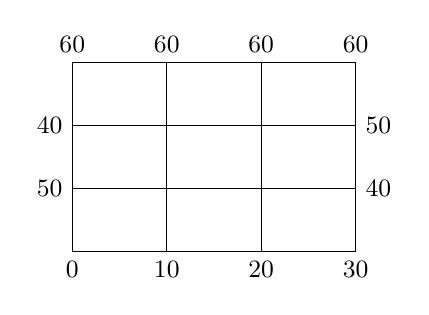
\begin{tikzpicture}[x=1.2cm,y=0.8cm]
 \foreach \i in {0,1,2,3}{\draw (\i,0)--(\i,3); \draw (0,\i)--(3,\i);}
 \foreach \x in {0,1,2,3}{\node[above] at (\x,3) {\small 60};}
 \node[left] at (0,2) {\small 40}; \node[left] at (0,1) {\small 50}; \node[right] at (3,2) {\small 50}; \node[right] at (3,1) {\small 40};
 \node[below] at (0,0) {\small 0}; \node[below] at (1,0) {\small 10}; \node[below] at (2,0) {\small 20}; \node[below] at (3,0) {\small 30};
\end{tikzpicture}} & 8 & -- & --\\ \hline
\end{seeB}
\end{seepaper}

%%%%%%%%%%%%%%%%%%%%%%%%%%%%%%%%%%%%%%%% WORK SYSTEMS DESIGN
% ---------------- IM233AI, Jan/Feb 2025
\begin{seepaper}
\paperinfo{code={IM233AI},examline={III Semester B.E. Regular/Supplementary Examinations Jan/Feb -- 2025},dept={Industrial Engineering and Management},title={WORK SYSTEMS DESIGN},time={03 Hours},maxmarks={100}}
\seehead
\instrA{}
\seepartA
\begin{seeA}
\qaq{1}{1.1}{Illustrate the Pyramidal Structure of the work.}{02}{2}{1}
\qa{1.2}{Distinguish between internal element and external element in cycle time analysis.}{02}{4}{1}
\qa{1.3}{Enumerate the categories of worker machine systems based on the levels of operator attention required.}{02}{1}{2}
\qa{1.4}{Differentiate between snap back and cumulative timing methods.}{02}{4}{2}
\qa{1.5}{What is lean production?}{02}{2}{3}
\qa{1.6}{Why is an allowance added to the normal time to complete the standard time?}{02}{2}{2}
\qa{1.7}{Identify the broad categories of factors causing fatigue in workers.}{02}{2}{4}
\qa{1.8}{List any four techniques of Work Measurement.}{02}{1}{2}
\qa{1.9}{In the context of lean manufacturing what is production leveling?}{02}{2}{3}
\qa{1.10}{In lean manufacturing, \blank[1.5cm] refers to waste or non-value-adding activities, while \blank[1.5cm] refers to overburdening people or equipment.}{02}{2}{3}
\end{seeA}
\seepart{PART-B}
\begin{seeB}
\qb{2}{a}{Distinguish between Production and Productivity. Also justify the rationale for considering labor productivity as a measure of organizational efficiency and effectiveness.}{08}{4}{1}
 & b & The normal time to perform a repetitive manual task is 4.25 minutes. In addition, an irregular work element whose normal time is 1.75 minutes must be performed every 8 cycles. Two work units are produced each cycle. The PFD allowance is 16\%. Determine the standard time per piece. How many work units are produced in an 8-hour shift at standard performance? Determine the anticipated amount of time worked and the amount of time lost per 8-hour shift that corresponds to the PFD allowance factor of 16\%. & 08 & 3 & 2\\ \hline
\qb{3}{a}{Review the applicability of three categories of Charting / diagrammatic techniques used by industrial engineers for collecting, displaying and analyzing data on a given work system.}{08}{2}{1}
 & b & Provide an overview on any four techniques of Methods Engineering. & 08 & 2 & 1\\ \hline
\orrow
\qb{4}{a}{Enumerate and provide a brief note on the principles of motion economy.}{09}{2}{1}
 & b & Review the phases involved in the systematic approach that can be used to accomplish a methods engineering study. & 07 & 2 & 1\\ \hline
\qb{5}{a}{What is a Work Element? Mention at least six guidelines for defining work elements in direct time study. Supplement with appropriate explanation and examples.}{08}{3}{2}
 & b & The continuous timing method in direct time study was used to obtain the elemental times for a worker machine task as indicated. Element c is a machine controlled and the time is constant. Elements a, b, d, e and f are operator controlled and external to machine cycle and they are performance rated at 90\%. If the machine allowance is 12\% and worker PFD allowance is 8\%, determine the normal time and standard time for the work cycle.
\qtabc{|l|c|c|c|c|c|c|}{\hline Element & a & b & c & d & e & f\\\hline Observed Time (min) & 0.12 & 0.28 & 0.78 & 1.04 & 1.45 & 1.80\\\hline} & 08 & 3 & 2\\ \hline
\orrow
\qb{6}{a}{What is meant by PMTS? Distinguish between First level PMTS and Higher level PMTS on the basis of at least five characteristics.}{08}{2}{2}
 & b & Analyse the causes for variability in the observed work element times that occur from one work cycle to another work cycle. & 08 & 4 & 2\\ \hline
\qb{7}{a}{Enumerate the seven wastes as advocated by Taiichi Ohno in Lean Production philosophy. Explain any four in detail.}{10}{3}{3}
 & b & Distinguish between Push System of production control and Pull System of production control. Support your answer with an appropriate illustration. & 06 & 4 & 3\\ \hline
\orrow
\qb{8}{a}{In Toyota Production System a standardized work procedure for a given task has three components. What are they? Explain any two in detail.}{08}{2}{3}
 & b & Explain the role of Total Productive Maintenance (TPM) in automation with examples. & 08 & 2 & 3\\ \hline
\qb{9}{a}{Employees in an office environment report eye strain, fatigue, and discomfort. Analyse the physical work environment and recommend improvements.}{08}{3}{4}
 & b & What is ergonomics and explain its purpose in production systems. Discuss how ergonomics and human factors are connected to engineering. & 08 & 2 & 4\\ \hline
\orrow
\qb{10}{a}{Highlight on the concept of anthropometry and its importance in designing for the human body, with examples.}{08}{2}{4}
 & b & Describe how mechanics can be applied to the human body to enhance safety and efficiency in the workplace. & 08 & 2 & 4\\ \hline
\end{seeB}
\end{seepaper}

% ---------------- IM233AI, Oct/Nov 2024 (Supplementary)
\begin{seepaper}
\paperinfo{code={IM233AI},examline={III Semester B.E. Supplementary Examinations Oct/Nov -- 2024},dept={Industrial Engineering and Management},title={WORK SYSTEMS DESIGN},time={03 Hours},maxmarks={100}}
\seehead
\instrA{}
\seepartA
\begin{seeA}
\qaq{1}{1.1}{Illustrate pyramidal structure of work.}{02}{2}{1}
\qa{1.2}{What is meant by the term productivity?}{02}{2}{1}
\qa{1.3}{List the symbols used in traditional industrial engineering charting techniques.}{02}{1}{2}
\qa{1.4}{List any two objectives of methods engineering.}{02}{1}{2}
\qa{1.5}{Mention the elements of standard time for manual work.}{02}{1}{3}
\qa{1.6}{Expand the acronym MOST.}{02}{1}{3}
\qa{1.7}{What is meant by Autonomation?}{02}{2}{1}
\qa{1.8}{Mention the main activities involved in 5s.}{02}{1}{2}
\qa{1.9}{What is meant by the term Anthropometry?}{02}{1}{4}
\qa{1.10}{Distinguish between the terms: `Accident' and `Hazard'.}{02}{2}{4}
\end{seeA}
\seepart{PART-B}
\begin{seeB}
\qb{2}{a}{During the base year in a mill 326000 tons of steel were produced using 203,000 labor hours. In the next year, the output was 341,000 tonns using 246,000 labor hours. Determine the (i) Labor productivity ratio for the base year, (ii) Labor productivity ratio for the second year, (iii) Labor productivity index for the second year.}{10}{3}{1}
 & b & Categorize the excess non-productive activities. Write a brief note on each of the category. & 06 & 3 & 1\\ \hline
\qb{3}{a}{Enumerate the steps in systematic approach of methods engineering application for an improvement.}{10}{2}{2}
 & b & Evaluation of alternative improvement proposals is done considering two categories of features and specifications. Write a note on them. & 06 & 2 & 2\\ \hline
\orrow
\qb{4}{a}{Review the basic data collection tools and analysis techniques used for problem solving.}{10}{4}{2}
 & b & Illustrate and elaborate on automation migration strategy. & 06 & 3 & 2\\ \hline
\qb{5}{a}{Classify the methods to determine time standards. Support your explanation with an illustration for better clarity.}{10}{3}{3}
 & b & Illustrate/sketch the model indicating the factors that must be standardized before a standard time can be set for a task. & 06 & 3 & 3\\ \hline
\orrow
\qb{6}{a}{Enumerate the steps involved in direct time study procedure to arrive at standard time for a job/activity.}{--}{--}{--}
 & b & A regular cycle of work consists of three elements a, b, c. Element `d' is irregular element performed every five cycles. Using the following details; compute normal time and standard time for the work cycle, using an allowance factor of 15\%.
\qtabc{|l|c|c|c|c|}{\hline Work element & a & b & c & d\\\hline Observed time (min) & 0.56 & 0.25 & 0.50 & 1.10\\\hline Performance Rating (\%) & 100 & 80 & 110 & 100\\\hline} & -- & -- & --\\ \hline
\qb{7}{a}{Summarize the seven forms of `waste' that needs to be eliminated as advocated by Taiichi Ohno to make the production system lean.}{--}{--}{--}
 & b & What is meant by the term `Kaizen'? How is Kaizen implemented for achieving the goal of continuous improvement in lean systems? & -- & -- & --\\ \hline
\orrow
\qb{8}{a}{Distinguish between `push' and `pull' systems of production control. Support your explanation with an illustrative example.}{--}{--}{--}
 & b & Illustrate the structure of a lean production system and highlight the key elements. & -- & -- & --\\ \hline
\qb{9}{a}{Sketch the block diagram model of the interactions in a human-machine system. Provide a brief note on different elements in the system.}{--}{--}{--}
 & b & Write a note on the primary casual factors for the occurrence of industrial accidents. & -- & -- & --\\ \hline
\orrow
\qb{10}{a}{Review the three broad topical areas of Ergonomics as a field of study.}{--}{--}{--}
 & b & Distinguish between `Single incident traumas' and `Cumulative trauma disorders' in the context of Ergonomics. & -- & -- & --\\ \hline
\end{seeB}
\end{seepaper}

% ---------------- IM233AI, April/May 2024
\begin{seepaper}
\paperinfo{code={IM233AI},examline={III Semester B.E. Examinations April/May -- 2024},dept={Industrial Engineering and Management},title={WORK SYSTEMS DESIGN},time={03 Hours},maxmarks={100}}
\seehead
\instrA{}
\seepartA
\begin{seeA}
\qaq{1}{1.1}{Illustrate the pyramidal structure of work.}{02}{2}{1}
\qa{1.2}{Define the term ``Productivity''.}{02}{1}{1}
\qa{1.3}{Distinguish between ``Methods Design'' and ``Methods Analysis''.}{02}{2}{2}
\qa{1.4}{One of the approaches for dealing with the automation projects in methods engineering is USA principle. Expand the acronym `USA'.}{02}{1}{2}
\qa{1.5}{What is meant by application speed ratio in the context of work measurement?}{02}{2}{3}
\qa{1.6}{Expand the acronym `MOST'.}{02}{1}{3}
\qa{1.7}{What is the principal objective of JIT?}{02}{2}{2}
\qa{1.8}{What does the term `Jidoka' refer to?}{02}{1}{2}
\qa{1.9}{List the four primary variables that influence the climate in the work place environment.}{02}{1}{4}
\qa{1.10}{Distinguish between the terms, ``industrial accident'' and ``hazard''.}{02}{2}{4}
\end{seeA}
\seepart{PART-B}
\begin{seeB}
\qb{2}{a}{Distinguish between the terms, `basic productive work content' and `excess non-productive work content.' Also illustrate with two examples for each category of excess non-productive activities that add to total task time.}{08}{3}{1}
 & b & A work group of 5 workers in a certain month produced 500 units of output working 8 hrs/day for 22 days in a month. Suppose in the next month, the same work group produced 600 units but were only 20 work days in the month. Using labor productivity measure, determine the productivity index using the prior month as a base. & 08 & 4 & 1\\ \hline
\qb{3}{a}{Enumerate the steps in a systematic approach that can be used to accomplish a methods engineering study.}{08}{2}{2}
 & b & Summarize the features and applicability of the following tools used by industrial engineers for basic data collection and analysis as part of problem solving process. (i) Defect concentration diagram (ii) Scatter diagram & 08 & 3 & 2\\ \hline
\orrow
\qb{4}{a}{Enumerate any eight principles of motion economy related to the use of human body.}{--}{--}{--}
 & b & Illustrate the automation migration strategy and explain the three phases included in the typical strategy followed by manufacturing organizations. & -- & -- & --\\ \hline
\qb{5}{a}{Depict a model indicating the factors that must be standardized before a standard time can be set for a task. Also explain the elements of the model.}{--}{--}{--}
 & b & The observed element times and performance ratings collected in a direct time study are indicated in the table below. The snapback/flyback timing method was used. The PFD allowance is 14\%. All the elements are regular elements in the work cycle. Determine: (i) Normal time and (ii) The standard time for the cycle.
\qtabc{|l|c|c|c|c|}{\hline Work Element & a & b & c & d\\\hline Observed time (min) & 0.22 & 0.41 & 0.30 & 0.37\\\hline Performance Rating (\%) & 90 & 120 & 100 & 90\\\hline} & -- & -- & --\\ \hline
\orrow
\qb{6}{a}{Examine the three sequence (activity sequence) models in Basic MOST and indicate the standard sequence of model parameters for each.}{--}{--}{--}
 & b & The snapback timing method was used in a direct time study of a task that includes a machine cycle. Elements a, b, c and d are performed by the operator and element `m' is a machine element; Element `b' is an internal element performed by the operator simultaneously with element `m'; and element `d' is an irregular element performed once every 15 cycles. Observed times and performance ratings are given in the table. The PFD allowance factor is 15\%, and the machine allowance is 20\%. Determine: (i) Normal time and (ii) Standard time for the work cycle.
\qtabc{|l|c|c|c|c|}{\hline Worker element & a & b & c & d\\\hline Observed time (min) -- manual & 0.22 & 0.65 & 0.47 & 0.75\\\hline Performance rating (\%) & 100 & 80 & 100 & 100\\\hline Machine element & & m & & \\\hline Observed time (min) -- machine & idle & 1.56 & idle & idle\\\hline} & -- & -- & --\\ \hline
\qb{7}{a}{Illustrate the structure of a lean production system and explain in detail any two ingredients of the system.}{--}{--}{--}
 & b & Examine the three prerequisites for successful implementation of Just-in-Time production system. & -- & -- & --\\ \hline
\orrow
\qb{8}{a}{Examine any four aspects influencing the stable and reliable production operations in a manufacturing environment.}{--}{--}{--}
 & b & Motivated workers participation in continuous improvement is critical for achieving the objective of lean production system. In the above context, discuss the relevance of visual management and 5s. & -- & -- & --\\ \hline
\qb{9}{a}{Depict the model of interactions in a typical human machine system. Provide an overview of the human components of interest in the system.}{08}{3}{4}
 & b & Work is performed in an environment that includes both physical and social aspects. Classify the broad categories into which physical environment can be segregated from ergonomics perspective. Elaborate on any two categories in detail. & 08 & 4 & 4\\ \hline
\orrow
\qb{10}{a}{Elucidate the three factors commonly identified in the ergonomics literature as the primary reasons for occurrence of industrial accidents.}{08}{2}{4}
 & b & Describe any four common cumulative trauma and other occupational disorders in a chosen sector of your interest. & 08 & 4 & 4\\ \hline
\end{seeB}
\end{seepaper}

% ---------------- IM233AI, Model Question Paper (2022 scheme)
\begin{seepaper}
\paperinfo{code={IM233AI},examline={III Semester B.E. Examinations April -- 2024 \\ MODEL QUESTION PAPER (2022 SCHEME)},dept={Industrial Engineering and Management},title={WORK SYSTEMS DESIGN},time={03 Hours},maxmarks={100}}
\seehead
\instrA{}
\seepartA
\begin{seeA}
\qaq{1}{1.1}{Distinguish between the terms: Production and Productivity.}{02}{--}{--}
\qa{1.2}{Classify the types of Worker-Machine Systems.}{02}{--}{--}
\qa{1.3}{Categorize the features and specifications to be considered in selecting among alternative improvement proposals in Methods Engineering.}{02}{--}{--}
\qa{1.4}{Expand the acronym USA in the context of methods engineering and automation.}{02}{--}{--}
\qa{1.5}{What is meant by the term Application Speed Ratio?}{02}{--}{--}
\qa{1.6}{Mention the prerequisites of Standard Time.}{02}{--}{--}
\qa{1.7}{What is meant by Lean Production System?}{02}{--}{--}
\qa{1.8}{Distinguish between Pull System and Push System of Production Control.}{02}{--}{--}
\qa{1.9}{List the three categories of Human-Machine Systems.}{02}{--}{--}
\qa{1.10}{What is meant by Anthropometry?}{02}{--}{--}
\end{seeA}
\seepart{PART-B}
\begin{seeB}
\qb{2}{a}{Distinguish between basic productive work environment and Excess non productive work environment. Also classify the excess non productive activities into three categories. Support your explanation with examples for each category.}{08}{--}{--}
 & b & The normal time for a repetitive task that produces two work units per cycle is 3.0 minutes. The plant uses a PFD allowance factor of 15\%. Determine (a) the standard time per piece and (b) how many work units are produced in an 8 hour shift at standard performance. & 08 & -- & --\\ \hline
\qb{3}{a}{Review any two categories of specialized analysis techniques used in Methods Engineering that are exclusive to operations analysis and industrial engineering.}{08}{--}{--}
 & b & Identify and explain the types of symbols used in a flow process chart. & 08 & -- & --\\ \hline
\orrow
\qb{4}{a}{Describe any two basic data collection and analysis techniques used in Methods Engineering.}{08}{--}{--}
 & b & Enumerate the principles of motion economy related to the design of tooling and equipment. & 08 & -- & --\\ \hline
\qb{5}{a}{Discuss the characteristics typical of industrial situations in which time standards would be beneficial?}{08}{--}{--}
 & b & The standard time is to be established for a manual work cycle by direct time study. The observed time for the cycle averaged 4.80 minutes. The worker's performance was rated at 90\% on all cycles observed. After eight cycles, the worker must exchange parts containers, which took 1.60 minutes, rated at 120\%. The PFD allowance for this class of work is 15\%. Determine (a) normal time and standard time (b) worker's efficiency if the worker produces 123 work units during an 8 hour shift. & 08 & -- & --\\ \hline
\orrow
\qb{6}{a}{Summarize different varieties of Predetermined Motion Time Systems.}{08}{--}{--}
 & b & Review different versions of MOST work measurement packages. & 08 & -- & --\\ \hline
\qb{7}{a}{Provide a historical note on the Lean Production Philosophy.}{08}{--}{--}
 & b & With the help of an illustration, explain the working of a kanban system between work stations. & 08 & -- & --\\ \hline
\orrow
\qb{8}{a}{Explain any two aspects of Autonomation with suitable examples.}{08}{--}{--}
 & b & What is Standardized Work Procedure? Explain the components of the same for a given task. & 08 & -- & --\\ \hline
\qb{9}{a}{What is human machine system? Review the two main components of the same.}{08}{--}{--}
 & b & Discuss the components of Physical work environment. & 08 & -- & --\\ \hline
\orrow
\qb{10}{a}{What is an industrial accident? Analyze the causes for the same from ergonomics perspective.}{08}{--}{--}
 & b & Describe any four common occupational diseases along with necessary causes. & 08 & -- & --\\ \hline
\end{seeB}
\end{seepaper}

%%%%%%%%%%%%%%%%%%%%%%%%%%%%%%%%%%%%%%%% MANUFACTURING PROCESSES
% ---------------- 21IM34, June/July 2025 (Supplementary)
\begin{seepaper}
\paperinfo{code={21IM34},examline={III Semester B.E. Supplementary Examinations June/July -- 2025},dept={Industrial Engineering and Management},title={MANUFACTURING PROCESS},time={03 Hours},maxmarks={100}}
\seehead
\instrA{}
\seepartA
\begin{seeA}
\qaq{1}{1.1}{Differentiate between job and batch production.}{02}{1}{1}
\qa{1.2}{Why is casting considered suitable for complex shapes?}{02}{1}{1}
\qa{1.3}{List the two common applications of rolling.}{02}{2}{2}
\qa{1.4}{What is the principle behind centrifugal casting?}{02}{2}{2}
\qa{1.5}{When would you choose adhesive bonding over welding?}{02}{3}{3}
\qa{1.6}{Suggest ways to reduce welding defects in MIG welding.}{02}{3}{3}
\qa{1.7}{What type of machining would you use for a flat surface with key slots?}{02}{2}{2}
\qa{1.8}{Why is excessive cutting temperature harmful?}{02}{2}{2}
\qa{1.9}{Why are advanced machining processes needed in modern manufacturing?}{02}{2}{2}
\qa{1.10}{Suggest a product where LBM is suitable.}{02}{2}{2}
\end{seeA}
\seepart{PART-B}
\begin{seeB}
\qb{2}{a}{Discuss the recent developments in manufacturing and their significance.}{08}{1}{1}
 & b & List the advantages and limitations of Expendable-Mould Casting Processes. & 08 & 2 & 2\\ \hline
\qb{3}{a}{Compare hot working and cold working process.}{08}{2}{2}
 & b & What is press forging? How does it differ from drop forging? & 08 & 2 & 2\\ \hline
\orrow
\qb{4}{a}{Describe the principle of Investment Casting and list its application.}{08}{3}{3}
 & b & Explain the steps of centrifugal casting process with a neat sketch. & 08 & 3 & 3\\ \hline
\qb{5}{a}{Which fusion-welding process would you select for welding thick steel plates, and why?}{08}{3}{3}
 & b & Evaluate how poor weldability can affect the quality and performance of a welded structure. & 08 & 3 & 3\\ \hline
\orrow
\qb{6}{a}{Explain the process of soldering and identify its common areas of application.}{08}{4}{4}
 & b & List and discuss welding defects and with their causes. & 08 & 4 & 4\\ \hline
\qb{7}{a}{Explain the role of built-up edge in the cutting process and how it affects machining performance.}{--}{--}{--}
 & b & State assumptions of merchant circle diagram with a neat sketch. & -- & -- & --\\ \hline
\orrow
\qb{8}{a}{List and describe the various tool angles used in single-point cutting tools.}{--}{--}{--}
 & b & Explain the significance of tool life in metal cutting operations and its effect on production cost and quality. & -- & -- & --\\ \hline
\qb{9}{a}{Which advanced machining process would you recommend for machining intricate holes in hard metals without tool wear? Justify your choice.}{--}{--}{--}
 & b & Explain the working principle of Electrochemical Machining (ECM). How is it different from conventional? & -- & -- & --\\ \hline
\orrow
\qb{10}{a}{Discuss the limitations of Abrasive-Jet Machining (AJM) for precision machining applications.}{--}{--}{--}
 & b & Explain the concept of hybrid machining. Why is it used instead of conventional or single advanced processes? & -- & -- & --\\ \hline
\end{seeB}
\end{seepaper}

% ---------------- IM234AI, Feb/Mar 2025
\begin{seepaper}
\paperinfo{code={IM234AI},examline={III Semester B.E. Regular/Supplementary Examinations Feb/Mar -- 2025},dept={Industrial Engineering and Management},title={MANUFACTURING PROCESSES},time={03 Hours},maxmarks={100}}
\seehead
\instrA{}
\seepartA
\begin{seeA}
\qaq{1}{1.1}{Describe the importance of pattern color coding and provide examples.}{02}{1}{1}
\qa{1.2}{What are chaplets and describe their purpose in casting.}{02}{1}{2}
\qa{1.3}{Name the differences between hot working and cold working.}{02}{2}{2}
\qa{1.4}{What is precision investment casting and list its advantages.}{02}{1}{2}
\qa{1.5}{Define electron beam welding (EBW) and state where it is used.}{02}{1}{1}
\qa{1.6}{List the factors influencing the weldability.}{02}{1}{3}
\qa{1.7}{Write the different types of chips formed in metal cutting.}{02}{1}{2}
\qa{1.8}{What is machinability and list the factors that affect it.}{02}{1}{3}
\qa{1.9}{Find the machining time required for drilling a 25 mm hole through a 50 mm thick plate at 600 rpm with a feed rate of 0.2 mm/rev.}{02}{1}{3}
\qa{1.10}{Write about the purpose of indexing in milling.}{02}{1}{4}
\end{seeA}
\seepart{PART-B}
\begin{seeB}
\qb{2}{a}{Discuss recent developments in manufacturing.}{08}{2}{1}
 & b & Illustrate the steps involved in sand moulding process with neat sketch. & 08 & 3 & 2\\ \hline
\qb{3}{a}{Explain the process of forging and compare smith forging, drop forging and press forging process.}{08}{4}{2}
 & b & Explain the principle of extrusion, discuss its types according to direction of flow of materials and illustrate with a neat sketch. & 08 & 4 & 2\\ \hline
\orrow
\qb{4}{a}{Discuss the principle of shell moulding process with neat sketch.}{08}{2}{2}
 & b & Explain the hot chamber die casting process with neat sketch. & 08 & 4 & 2\\ \hline
\qb{5}{a}{Explain the principles of arc welding with basic welding circuit and its applications.}{08}{4}{1}
 & b & Identify the welding process that uses heat generated from burning a combination of different gases to melt and fuse metals and how does it work? Explain with neat sketch. & 08 & 4 & 1\\ \hline
\orrow
\qb{6}{a}{Distinguish between fusion welding and solid state welding with examples.}{--}{--}{--}
 & b & Discuss the factors affecting weld quality and explain the causes and remedies of common welding defects. & -- & -- & --\\ \hline
\qb{7}{a}{Explain single point cutting tool nomenclature and its geometry with neat sketch.}{--}{--}{--}
 & b & In an orthogonal cutting test with a tool of rake angle 10$^{\circ}$, the following observations were made: chip thickness ratio = 0.3, cutting force = 1290 N, feed force = 1650 N. From Merchant's theory, calculate shear plane angle, coefficient of friction, velocity of chip relative to tool at the chip tool interface. & -- & -- & --\\ \hline
\orrow
\qb{8}{a}{Explain the desired properties and types of cutting tool materials.}{--}{--}{--}
 & b & Discuss the different types of cutting fluids and their application. & -- & -- & --\\ \hline
\qb{9}{a}{With a neat sketch, explain the nomenclature of twist drill bit.}{--}{--}{--}
 & b & Explain the different types of drilling related operations with neat sketch. & -- & -- & --\\ \hline
\orrow
\qb{10}{a}{With neat sketch, differentiate between up milling and down milling operation.}{--}{--}{--}
 & b & A gear blank on the milling machine in order to cut 73 teeth, differential indexing is used to rotate the part. The machine has a 40:1 ratio index head. Calculate the gear ratio necessary between the spindle and index plate. & -- & -- & --\\ \hline
\end{seeB}
\end{seepaper}

% ---------------- IM234AI, April/May 2024
\begin{seepaper}
\paperinfo{code={IM234AI},examline={III Semester B.E. Examinations April/May -- 2024},dept={Industrial Engineering and Management},title={MANUFACTURING PROCESSES},time={03 Hours},maxmarks={100}}
\seehead
\instrA{}
\seepartA
\begin{seeA}
\qaq{1}{1.1}{The value of chip reduction coefficient depends upon cutting tool material and \blank[1.8cm].}{2}{1}{1}
\qa{1.2}{In the Taylor's tool life equation, $VT^n = C$, the value of n = 0.5. The tool life has 180 minutes at a cutting speed of 18 m/min. If the tool life is reduced to 45 minutes, then the cutting speed will be \blank[1.5cm].}{2}{3}{3}
\qa{1.3}{The working of tin and lead even at room temperature is termed as hot working. Give reasons.}{2}{3}{2}
\qa{1.4}{List any two defects of welding.}{2}{2}{2}
\qa{1.5}{State any two differences between orthogonal cutting and oblique cutting.}{2}{2}{1}
\qa{1.6}{Define porosity.}{2}{2}{3}
\qa{1.7}{List any two limitations of extrusion process.}{2}{1}{2}
\qa{1.8}{List any two applications of hydro forming process.}{2}{3}{1}
\qa{1.9}{Circumference of a work piece is to be divided into 60 equal divisions using simple indexing method having 40 worm wheel teeth. Calculate indexing movement.}{2}{3}{2}
\qa{1.10}{List the cutting parameters that greatly affects the tool life.}{2}{2}{2}
\end{seeA}
\seepart{PART-B}
\begin{seeB}
\qb{2}{a}{Define pattern. List the types of patterns and explain any one briefly.}{06}{2}{2}
 & b & Explain the process of casting with a neat sketch. & 10 & 1 & 1\\ \hline
\qb{3}{a}{With a neat sketch, explain the centrifugal casting process which is best suited for casting of hollow pipes and tubes.}{10}{3}{3}
 & b & List the advantages and disadvantages of extrusion process. & 06 & 2 & 2\\ \hline
\orrow
\qb{4}{a}{How are cup shaped vessels being manufactured? Explain the metal spinning process with a neat sketch.}{10}{3}{3}
 & b & List the advantages and disadvantages of hydro forming process. & 06 & 2 & 2\\ \hline
\qb{5}{a}{With a neat sketch, explain resistance seam welding process which is best used to rectangular or square or even in circular shapes.}{--}{--}{--}
 & b & State the differences between fusion and solid state welding processes. & -- & -- & --\\ \hline
\orrow
\qb{6}{a}{Explain with the help of sketch, working principle of Thermit welding.}{--}{--}{--}
 & b & What is weld quality? Explain the factors that affect weldability. & -- & -- & --\\ \hline
\qb{7}{a}{List cutting tool materials. Describe in brief, stating its principal characteristics and applications of any two cutting tool materials.}{--}{--}{--}
 & b & Derive an expression for the shear angle in orthogonal cutting in terms of rake angle and chip thickness ratio. & -- & -- & --\\ \hline
\orrow
\qb{8}{a}{What are the different types of chips that are formed in metal machining?}{--}{--}{--}
 & b & An orthogonal cutting operation is performed using a rake angle of 15$^{\circ}$, chip thickness before the cut = 0.012 inch and width of cut = 0.100 inch. The chip thickness ratio is measured after the cut to be 0.55. Determine (i) the chip thickness after the cut (ii) Shear angle (iii) Friction angle (iv) Coefficient of friction (v) Shear strain. & -- & -- & --\\ \hline
\qb{9}{a}{Define indexing. Explain the following indexing methods. (i) Direct indexing (ii) Compound indexing.}{--}{--}{--}
 & b & A drilling operation is performed on a workpiece made of mild steel using a twist drill with a diameter of 10 mm. The cutting speed is set to 60 m/min and the feed rate is 0.1 mm/rev. The drill needs to penetrate the workpiece to a depth of 30 mm. Assume that the drill needs to be changed after every 50 holes and each tool change takes 2 minutes. Calculate the total machining time required to drill 200 holes in the workpiece. & -- & -- & --\\ \hline
\orrow
\qb{10}{a}{State different types of drilling operations and explain any two with a neat sketch.}{--}{--}{--}
 & b & Differentiate between up milling and down milling. & -- & -- & --\\ \hline
\end{seeB}
\end{seepaper}

%%%%%%%%%%%%%%%%%%%%%%%%%%%%%%%%%%%%%%%% DIGITAL METROLOGY
% ---------------- IM235AI, Feb/Mar 2025
\begin{seepaper}
\paperinfo{code={IM235AI},examline={III Semester B.E. Regular/Supplementary Examinations Feb/Mar -- 2025},dept={Industrial Engineering and Management},title={DIGITAL METROLOGY},time={03 Hours},maxmarks={100}}
\seehead
\instrA{}
\seepartA
\begin{seeA}
\qaq{1}{1.1}{Differentiate between Static and Dynamic Characteristics of a measurement system.}{02}{2}{1}
\qa{1.2}{State the importance of calibration in a measurement system.}{02}{1}{1}
\qa{1.3}{List any four key specifications of a sensor.}{02}{1}{2}
\qa{1.4}{Mention the main components of a data acquisition system.}{02}{1}{2}
\qa{1.5}{Define tolerance.}{02}{1}{3}
\qa{1.6}{Highlight any two functions of optical flats.}{02}{2}{3}
\qa{1.7}{What is meant by Fit?}{02}{1}{3}
\qa{1.8}{What is the Root Mean Square (RMS) value in surface finish measurement?}{02}{1}{3}
\qa{1.9}{Mention the type of CMM which is best suited for inspecting large and heavy workpieces.}{02}{2}{4}
\qa{1.10}{State the primary use of a laser in laser metrology.}{02}{2}{4}
\end{seeA}
\seepart{PART-B}
\begin{seeB}
\qb{2}{a}{Explain the elements of a generalized measurement system with a neat sketch.}{08}{2}{1}
 & b & Explain the importance of calibration in measurement systems. & 08 & 2 & 1\\ \hline
\qb{3}{a}{Explain the working of a potentiometer as a displacement sensor.}{08}{3}{2}
 & b & State and discuss the working principle of a tacho generator. & 08 & 3 & 2\\ \hline
\orrow
\qb{4}{a}{Discuss the working of piezoelectric sensors for pressure measurement.}{08}{3}{2}
 & b & Explain the elements of a data acquisition system and the role of A/D and D/A converters. & 08 & 2 & 2\\ \hline
\qb{5}{a}{With suitable examples, differentiate between interchangeability and selective assembly.}{08}{3}{3}
 & b & Differentiate between the hole basis system and the shaft basis system. Identify which is more commonly preferred, and provide the fits designation as per IS 919 -- 1963. & 08 & 3 & 3\\ \hline
\orrow
\qb{6}{a}{Explain the significance of tolerance in manufacturing. Discuss the various types of tolerances.}{--}{--}{--}
 & b & What is Geometric Dimensioning and Tolerancing (GD\&T)? And elaborate on the concept of position tolerance. & -- & -- & --\\ \hline
\qb{7}{a}{Explain the gear tooth Vernier method used to measure the thickness of gear teeth.}{--}{--}{--}
 & b & Discuss the application of optical flats in interferometry for flatness measurement. & -- & -- & --\\ \hline
\orrow
\qb{8}{a}{With the help of a neat sketch, explain the working and applications of a Tool Maker's Microscope.}{--}{--}{--}
 & b & Elaborate on the use of Tomlinson Surface Meter in measuring surface finish. & -- & -- & --\\ \hline
\qb{9}{a}{Describe the constructional features and working principle of a Coordinate Measuring Machine.}{--}{--}{--}
 & b & Explain the role of digital devices in computer-aided inspection with a Coordinate Measuring Machine. & -- & -- & --\\ \hline
\orrow
\qb{10}{a}{Identify the different types of Coordinate Measuring Machine (CMMs) and their specific applications.}{--}{--}{--}
 & b & Mention the principle and applications of the Michelson Interferometer in laser metrology. & -- & -- & --\\ \hline
\end{seeB}
\end{seepaper}

% ---------------- IM235AI, April 2024
\begin{seepaper}
\paperinfo{code={IM235AI},examline={III Semester B.E. Examinations Apr -- 2024},dept={Industrial Engineering and Management},title={DIGITAL METROLOGY},time={03 Hours},maxmarks={100}}
\seehead
\instrA{}
\seepartA
\begin{seeA}
\qaq{1}{1.1}{Discuss the differences between static and dynamic characteristics of a measurement system.}{02}{1}{1}
\qa{1.2}{List the Errors in measurements.}{02}{2}{2}
\qa{1.3}{Explain the functioning of a Piezoelectric Sensor and provide example for its applications.}{02}{2}{2}
\qa{1.4}{List the applications of a Capacitive Transducer in Proximity Sensing.}{02}{2}{2}
\qa{1.5}{What is meant by ``Basic Hole'' and ``Basic Shaft''?}{02}{2}{3}
\qa{1.6}{How will you write the fit: Shaft `m' of grade 5 and hole `H' of grade 11 and the basic size of 40 mm?}{02}{1}{3}
\qa{1.7}{An optical flat can be employed to measure height differences in which range?}{02}{2}{2}
\qa{1.8}{Describe the working principle of an Autocollimator.}{02}{1}{2}
\qa{1.9}{Describe the working principle of a Michelson Interferometer.}{02}{2}{4}
\qa{1.10}{List four applications of Laser Metrology in Industry.}{02}{2}{4}
\end{seeA}
\seepart{PART-B}
\begin{seeB}
\qb{2}{a}{Enumerate on the generalized measurement system. Justify the answer with an example, neat sketches and block diagrams.}{08}{3}{1}
 & b & Describe briefly the working principle of a Capacitive Transducer and also explain the measurement of linear displacement in a surface using the change in the area of plates. & 08 & 2 & 1\\ \hline
\qb{3}{a}{Discuss the specifications of sensors and their importance in metrology. Elucidate various types of sensors employed in measurement procedures.}{08}{3}{2}
 & b & Explain the Velocity and motion sensors and their application in metrology for the detection of infrared radiation and temperature variations. & 08 & 2 & 2\\ \hline
\orrow
\qb{4}{a}{Describe the factors influencing the selection of sensors for a particular application. How can one ensure the compatibility between sensors and data acquisition systems?}{08}{3}{2}
 & b & Compare and contrast position sensors and proximity sensors, highlighting their working principles and applications. & 08 & 3 & 2\\ \hline
\qb{5}{a}{In a limit system the following limits are specified to give a clearance fit between a shaft and a hole: Shaft 30 ${}^{-0.005}_{-0.018}$ mm$\phi$; Hole 30 ${}^{+0.020}_{-0.000}$ mm$\phi$. Determine: (i) Basic size (ii) Shaft and hole tolerances (iii) The shaft and hole limits (iv) The maximum and minimum clearance.}{08}{--}{--}
 & b & Define Fit. Explain briefly the various types of fits with examples. & 08 & -- & --\\ \hline
\orrow
\qb{6}{a}{Enumerate on the concept: (i) Interchangeability (ii) Hole basis systems.}{--}{--}{--}
 & b & Design the `General' type `GO' and `NOGO' gauges for the components having 50H8c8 fit. Given the following with usual notations: (i) Upper deviation for Shaft = (95 + 0.8D) microns (ii) 50 mm falls in the diameter step of 50 -- 80 mm (iii) IT8 = 25i. Take wear allowance as 10\% of the gauge Tolerance. Also mention the type of fit. Represent the dimensions graphically. & -- & -- & --\\ \hline
\qb{7}{a}{Enumerate on the working of a floating carriage micrometer and explain how the minor and effective diameter of a screw thread can be measured.}{--}{--}{--}
 & b & With the help of a neat sketch briefly explain the method of determining the chordal thickness of a gear tooth using gear tooth Vernier Calliper. & -- & -- & --\\ \hline
\orrow
\qb{8}{a}{Explain the constant chord method for measuring the gear tooth thickness.}{--}{--}{--}
 & b & Describe briefly the working principle of a Tool Makers Microscope and explain how the minor and effective diameter of a screw thread can be measured. & -- & -- & --\\ \hline
\qb{9}{a}{Enumerate on the different types of main structure of a Coordinate Measuring Machine with neat sketches, and list out the industrial applications of a CMM.}{--}{--}{--}
 & b & Describe briefly the working of a Michelson Interferometer and list out its applications. & -- & -- & --\\ \hline
\orrow
\qb{10}{a}{Describe the role of CMM in Computer Aided Manufacturing and explain briefly the advantages of CMM.}{--}{--}{--}
 & b & Explain the basic principle of LASER. List the various uses of LASER in metrology and explain any two in detail. & -- & -- & --\\ \hline
\end{seeB}
\end{seepaper}

% ---------------- IM235AI, Model Question Paper (2022 scheme)
\begin{seepaper}
\paperinfo{code={IM235AI},examline={III Semester B.E. Examinations \\ MODEL QUESTION PAPER (2022 SCHEME)},dept={Industrial Engineering and Management},title={DIGITAL METROLOGY},time={03 Hours},maxmarks={100}}
\seehead
\instrA{}
\seepartA
\begin{seeA}
\qaq{1}{1.1}{List any two desirable static and dynamic characteristics of measuring instruments.}{02}{2}{1}
\qa{1.2}{Mention the working principle of an Inductive sensor.}{02}{1}{2}
\qa{1.3}{Categorize the two applications of a Tactile sensor and analyze the principles underlying the use of tactile sensors in each application.}{02}{3}{2}
\qa{1.4}{Identify the two techniques used for converting Digital Signals into Analog signals.}{02}{2}{2}
\qa{1.5}{Compare and contrast the Hole basis system and shaft basis system in terms of their application in geometric dimensioning and tolerancing (GD\&T).}{02}{3}{1}
\qa{1.6}{Define Maximum clearance and Fundamental deviation.}{02}{1}{1}
\qa{1.7}{Evaluate the importance of optical flats in measuring surface finish, considering their role in precision measurement techniques.}{02}{3}{3}
\qa{1.8}{Evaluate the significance of determining a Ten-point Height Average Value in surface metrology.}{02}{3}{3}
\qa{1.9}{Classify the primary components of a Coordinate Measuring Machine (CMM) according to their functions.}{02}{2}{4}
\qa{1.10}{Classify the different geometrical checks performed on machine tools using LASER technology and analyze the principles behind each check.}{02}{3}{4}
\end{seeA}
\seepart{PART-B}
\begin{seeB}
\qb{2}{a}{Describe briefly the three stages of a generalized measurement system with block diagram. Provide two specific examples of measurement systems and identify how these examples demonstrate the three stages of measurement according to the categorized stages mentioned.}{08}{3}{1}
 & b & Illustrate the operational principles of two distinct resistive transducers, namely the strain gauge and the thermistor, and compare their applications in real-world scenarios. & 08 & 3 & 2\\ \hline
\qb{3}{a}{Explain the functioning of tactile sensors detailing its basic operation and how it detects contact with surfaces. Evaluate the advantages and limitations of this sensor in different scenarios, such as robotics, medical devices, touch-sensitive electronics, and industrial monitoring.}{08}{4}{2}
 & b & Describe the operational principles of Potentiometer Sensors based on resistance change. Explain how these sensors function to measure position, displacement, or angle by varying resistance. Provide examples of their applications in volume control knobs, servo motors, joysticks, and industrial position feedback systems. & 08 & 4 & 2\\ \hline
\orrow
\qb{4}{a}{Describe the operational principles of a tachogenerator and its role in measuring rotational speed. Evaluate the role of tachogenerators in measuring and monitoring rotational speed in automotive systems and automation/robotics.}{08}{4}{2}
 & b & Enumerate briefly on the classification of sensors based on different criteria and explain the working principle of Hall effect sensors. Discuss how Hall effect sensors generate a voltage difference in response to a magnetic field and how this principle is applied in various applications such as proximity sensing, position sensing, and speed measurement. & 08 & 4 & 2\\ \hline
\qb{5}{a}{Compare and contrast the characteristics, advantages, and applications of different types of fits in engineering assemblies. Also evaluate their suitability for specific assembly requirements.}{08}{4}{1}
 & b & Determine the actual dimension to be provided for a shaft and hole of 90 mm size for h8E9 type of fit. (i) Size 90 mm falls in the diameter step of 80 mm--100 mm. (ii) Value of tolerances for IT8 and IT9 are 25i and 40i. (iii) Value of fundamental deviation for `e' type shaft is 11D$^{0.41}$. Also mention the type of fit. Represent the dimensions graphically. & 08 & 4 & 1\\ \hline
\orrow
\qb{6}{a}{Explain briefly the Hole basis system and shaft basis system in geometric dimensioning and tolerancing (GD\&T). Analyze the principles behind each system, evaluate their advantages and limitations, and assess their effectiveness in ensuring proper fit and functionality in mechanical components, such as engine parts or aerospace components.}{08}{4}{1}
 & b & Enumerate on the concepts of interchangeability and selective assembly in manufacturing processes. How do these principles contribute to efficient production and product quality? Provide examples to illustrate your explanation. & 08 & 3 & 1\\ \hline
\qb{7}{a}{Apply the principle of interference to demonstrate the functioning of an autocollimator? Furthermore, discuss how autocollimators are practically utilized in manufacturing settings to assess the straightness of components.}{08}{4}{3}
 & b & Define Crest, Flank and Pitch and schematically represent on a screw thread. Explain how the major diameter of a screw thread can be measured using Bench micrometer. & 08 & 3 & 3\\ \hline
\orrow
\qb{8}{a}{Discuss the Tomlinson Surface Meter, its construction, principles of operation, and applications in surface finish measurement. Explain how this specialized instrument contributes to accurate surface finish analysis in engineering and manufacturing processes, highlighting its advantages and limitations.}{08}{4}{3}
 & b & Define Pitch Circle diameter, addendum and dedendum and represent on a gear profile. Assess the effectiveness of using vernier calipers for gear tooth thickness measurement compared to other measurement methods, and discuss potential sources of error in gear measurements. & 08 & 3 & 3\\ \hline
\qb{9}{a}{Explain briefly the 4 main elements of a Coordinate Measuring Machine (CMM). Evaluate how each component contributes to the accurate measurement and inspection capabilities of the CMM in various industrial applications.}{08}{3}{4}
 & b & How does Coordinate Measuring Machine (CMM) integration with Computer-Aided Manufacturing (CAM) enhance quality control processes in manufacturing? Discuss with examples. & 08 & 3 & 4\\ \hline
\orrow
\qb{10}{a}{Describe the key components of a laser interferometry system in detail, focusing on its different elements. Explain the function of each component and how they collectively enable precise distance measurements and displacement sensing through interference phenomena.}{08}{3}{4}
 & b & Analyze the components and functions of a control system integrated with a data conversion system. Provide a diagram illustrating signal flow and conversion between analog and digital formats. & 08 & 3 & 4\\ \hline
\end{seeB}
\end{seepaper}

% ---------------- 21IM52, Model Question Paper (2021 scheme)
\begin{seepaper}
\paperinfo{code={21IM52},examline={V Semester B.E. April -- 2024 Examinations \\ Model Question Paper (2021 Scheme)},dept={Industrial Engineering and Management},title={DIGITAL METROLOGY},time={03 Hours},maxmarks={100}}
\seehead
\instrA{}
\seepartA
\begin{seeA}
\qaq{1}{1.1}{Differentiate between static and dynamic errors in the context of measurements.}{02}{1}{1}
\qa{1.2}{Give two examples each for resistive and capacitive transducers.}{02}{2}{2}
\qa{1.3}{Differentiate between A/D and D/A converters in the context of a data acquisition system.}{02}{2}{2}
\qa{1.4}{Give two applications of velocity and motion sensors.}{02}{2}{2}
\qa{1.5}{Differentiate hole and shaft basis system.}{02}{2}{3}
\qa{1.6}{List the important types of fits.}{02}{1}{3}
\qa{1.7}{Give the working principle of optical flats and Tool Makers microscope.}{02}{2}{2}
\qa{1.8}{Define best size wire.}{02}{1}{2}
\qa{1.9}{List any four applications of CMM.}{02}{2}{4}
\qa{1.10}{Differentiate between bridge and gantry type CMM.}{02}{2}{4}
\end{seeA}
\seepart{PART-B}
\begin{seeB}
\qb{2}{a}{Discuss the components and functioning of the generalized measurement system, providing justification through an illustrative example, clear sketches, and block diagrams.}{08}{3}{1}
 & b & Describe briefly the working principle of a Capacitive Transducer and also explain the measurement of linear displacement in a surface using the change in the area of plates. & 08 & 2 & 1\\ \hline
\qb{3}{a}{Discuss the fundamental concept of sensors and their importance in metrology. Include examples to elucidate various types of sensors employed in measurement procedures.}{08}{3}{2}
 & b & Explain the operational principles of pyroelectric sensors and their application in metrology for the detection of infrared radiation and temperature variations. & 08 & 2 & 2\\ \hline
\orrow
\qb{4}{a}{Classify sensors based on their functionality into displacement, position, and proximity sensors. Discuss any one type, providing examples and applications in metrology.}{08}{3}{2}
 & b & Explain how piezoelectric sensors are employed for fluid pressure measurements in metrology. Provide examples of their usage and advantages in pressure sensing applications. & 08 & 3 & 2\\ \hline
\qb{5}{a}{Calculate the limits of tolerance and allowance for a 25 mm shaft and hole pair designated by H8d9 and sketch the fit. Given: 25 mm lies between 18 and 30, fundamental deviation of `H' hole = 0, fundamental deviation of `d' shaft = $-$16D$^{0.44}$, IT8 = 25i, IT9 = 40i.}{08}{4}{4}
 & b & Discuss the concepts of (i) Interchangeability and (ii) Selective Assembly, highlighting their significance in engineering and manufacturing processes. & 08 & 2 & 3\\ \hline
\orrow
\qb{6}{a}{Define the concept of fit and provide a concise overview of the different types of fits, supplemented with illustrative examples.}{08}{2}{3}
 & b & Calculate the relevant dimensions of 35H7f8 fit, dimension 35 falls in the steps of 30--50 mm. Fundamental deviation for f shaft is $-$5.5D$^{0.41}$, IT7 = 16i, IT8 = 25i. & 08 & 4 & 4\\ \hline
\qb{7}{a}{Illustrate the terminologies utilized to denote surface roughness through a clear diagram, elucidating each term's significance.}{08}{3}{2}
 & b & Illustrate the operational mechanism of a floating carriage micrometer using a clear diagram and provide a concise explanation of its functionality. & 08 & 2 & 2\\ \hline
\orrow
\qb{8}{a}{Enumerate and describe five frequently employed techniques for measuring surface roughness in engineering contexts.}{08}{3}{2}
 & b & Illustrate the operational principles of a tool maker's microscope through a clear diagram, providing a brief overview of its functionality. & 08 & 2 & 2\\ \hline
\qb{9}{a}{Illustrate and describe two variations of Coordinate Measuring Machines (CMMs) using sketches to elucidate their distinguishing features and operational methodologies.}{08}{2}{4}
 & b & Describe briefly the working of a Michelson Interferometer and list out its applications. & 08 & 2 & 3\\ \hline
\orrow
\qb{10}{a}{Discuss the significance and applications of Coordinate Measuring Machines (CMMs) in various industries.}{08}{3}{4}
 & b & Explain the fundamental principle underlying LASER technology. Enumerate the diverse applications of LASER in metrology and elaborate on two specific applications in depth. & 08 & 2 & 3\\ \hline
\end{seeB}
\end{seepaper}

\end{document}
